\documentclass[../a062main.tex]{subfiles}
\graphicspath{{\subfix{../figures/}}}

\begin{document}

\chapter{The Tools of Astronomy}
\section{Positions in Space}
We'll begin by studying how we can measure the position of an astronomical object in space.
There are two dimensions to consider: where the object appears in the night sky, and how far away it is from Earth.
We'll tackle each of these, starting with the first.

\subsection*{Celestial Coordinate Systems}
For now, it will be useful for us to imagine the sky as a ``\textbf{celestial sphere}'' that revolves around us, the radius of which is of no concern.
In order to specify the position of an object on this sphere we will need two coordinates: one that specifies the horizontal angle at which the object can be found, and another that specifies its height on the sphere.

There's a couple of natural ways in which we can assign these coordinates.
One is the \textbf{altitude-azimuth coordinate system}, which is defined with respect to the observer's local horizon.
The object's horizontal position, its \textbf{azimuth} $A$, is specified by the eastward angle from geographic north; its vertical position, its \textbf{altitude} $h$, is its angle above the horizon.
(Sometimes height is specified using the \textbf{zenith distance} $z$, which is measured downward from the highest point in the sky. $h + z = 90^\circ$.)
All angles are measured in degrees.

This coordinate system is great for casual observations, but not so much for cataloging---an object's altitude-azimuth coordinates will change over time due to movements of the Earth!
To combat this we can define a coordinate system with respect to Earth's equator, with quantities that are analagous to the familiar geographic coordiante system.
We can extend the equator outward onto the celestial sphere to create a \textbf{celestial equator}; similarly extending the poles gives the \textbf{celestial poles}.
The equivalent of longitude is called \textbf{right ascension} $\alpha$, and latitude becomes \textbf{declination} $\delta$.
This arrangement is called the \textbf{equatorial coordinate system}.

Declination is easy.
Objects that are above the celestial equator get a positive $\delta$ while those below get a negative $\delta$.
We usually write declinations using degrees, arcminutes, and arcseconds: there are sixty arcminutes in a degree ($1^\circ = 60'$) and sixty arcseconds in a arcminute ($1' = 60''$).

Right ascension is a little frustrating.
Looking down from the north celestial pole, we measure $\alpha$ counterclockwise (westward) from some reference point that we'll define soon.
We write right ascensions using hours, minutes, and seconds---which are distinct from arcseconds!
The celestial sphere is divided into 24 hours, so $1^\text{h} = 15^\circ$.
From there we again divide by sixty for each subdivision, so $1^\text{m} = 15'$ and $1^\text{s} = 15''$.
The logic here is to mirror the way we measure time as Earth rotates, but we just end up with needlessly confusing units.

Now, as Earth rotates, the Sun traces out a ``\textbf{great circle}'' around the celestial sphere called the \textbf{ecliptic}.
The highest and lowest points on the ecliptic are called the summer and winter solstices, respectively.
The points at which it crosses the celestial equator are called the vernal and autumnal equinoxes; the former occurs when the Sun is traveling upward, while the latter occurs while traveling downward.
We arbitrarily define the \textbf{vernal equinox} $\Upsilon$ to be our $\alpha = 0$ reference point for right ascension.

Alas, not even this equatorial coordiante system is perfect since the Earth really acts like a giant gyroscope with a precession period on the order of tens of thousands of years.
A better reference plane would be one defined by Earth's orbit around the Sun---we only stick with the equator because of institutional inertia.
For consistency, we usually record positions as they were at noon on January 1, 2000.
(We call this the \textbf{J2000.0 epoch}, using J for the Julian calendar whch astronomers use for its simplicity.)

\subsection*{Angular Separation}
With this understanding of the equatorial coordinate system, we can do some trigonometry to calculate the \textbf{angular separation} $\Delta \theta$ between two objects in the night sky.
Spherical trigonometry is hard, but if the objects we're considering are close enough together, we can approximate the triangle formed by $\Delta \theta$, $\Delta \delta$, and $\Delta \alpha$ as a planar right triangle that we can do trig with.

Suppose the celestial sphere has radius $R$.
(The choice of $R$ doesn't matter since we hope it'll cancel out in the end anyway.)
Obviously, the hypotenuse of this triangle is $R \Delta \theta$ and one of the legs is $R \Delta \delta$.
The leg due to the right ascension, however, is not $R \Delta \alpha$ because the rings of right ascension get smaller as they get closer to the poles.
The radius of this ring is $R \cos \delta$, where $\delta$ is any declination between the two objects we're considering.
(The precise value is unimportant in our approximation.)
So the leg we really want is $R \cos \delta \,\Delta \alpha$, and by the Pythagorean theorem we can write
\begin{align*}
    (R \Delta \theta)^2 &= (R \Delta \delta)^2 + (R \cos \delta \,\Delta \alpha)^2 \\
    (\Delta \theta)^2 &= (\Delta \delta)^2 + (\cos \delta \,\Delta \alpha)^2,
\end{align*}
where $\delta$ and $\alpha$ have the same units (usually degrees or arcseconds).
This gives the angular separation between the objects!

\subsection*{Trigonometric Parallax}
We'll now turn to the second question we posed at the beginning of this section, the question of distance.
We can measure distances to relatively nearby stars using the method of \textbf{stellar parallax}.
As the Earth orbits around the Sun, these stars appear to move back and forth very slightly relative to background stars, as shown below.
\begin{center}
    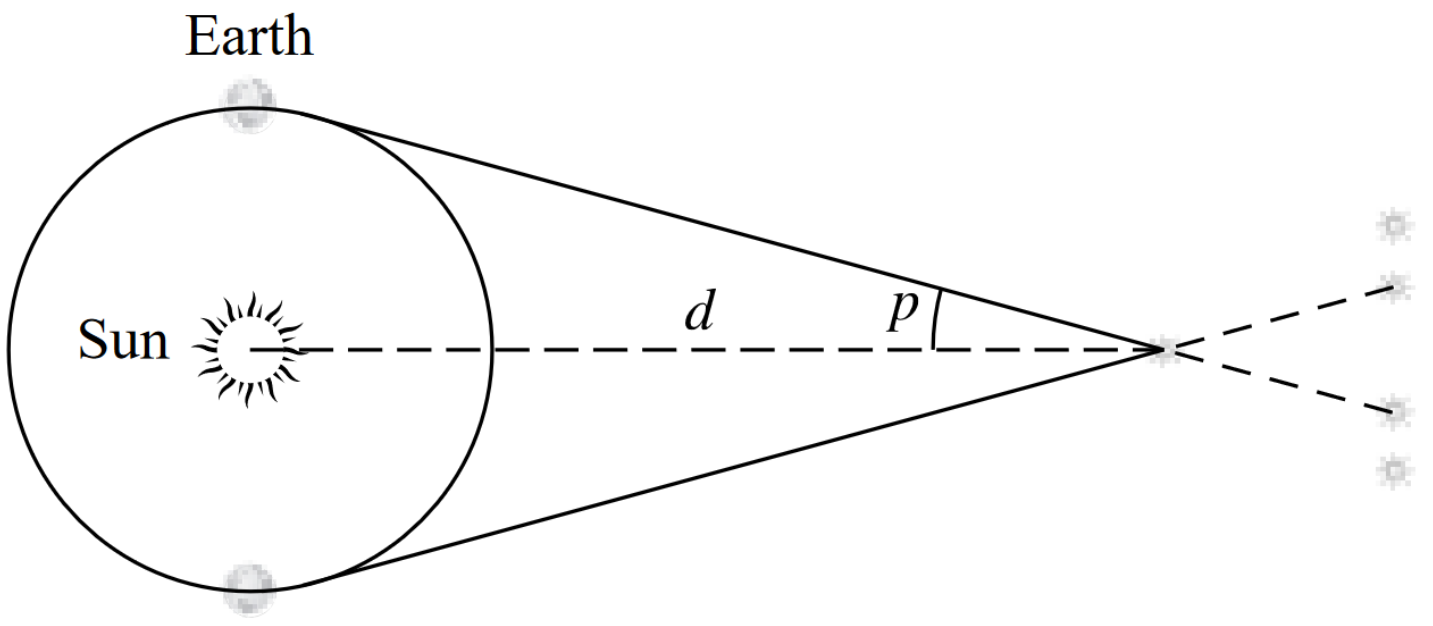
\includegraphics[width=0.55\textwidth]{stellarParallax.png}
\end{center}
The angle $p$ is called the \textbf{parallax angle}.
The distance between the Earth and the Sun is known to be one astronomical unit (AU), so we can use trigonometry to determine the distance $d$ to the star:
\[ \tan p = \frac{1 \text{ AU}}{d}. \]
Applying the small-angle approximation $\tan p \approx p$ gives
\[ \boxed{d = \frac{1}{p} \text{ AU}}, \]
where $p$ is measured in radians.
However, $p$ is often given in arcseconds, which is a little unweildy here.
To make things simpler, we can define the \textbf{parsec} (pc), which is the distance to a star whose parallax angle is $1''$.
So the conversion from radians to arcseconds gives
\[ \boxed{d = \frac{1}{p} \text{ pc}}, \]
where $p$ is measured in arcseconds.

\section{The Two-Body Problem}
\subsection*{The Planar Restricted Two-Body Problem}
Consider a star with mass $M_\star$ about which a planet with mass $m$ orbits.
The star is positioned at the origin, and the planet has position $\mbf{r}$ and velocity $\mbf{v}$.
Notice that all of the interactions between the star and planet occur in the same plane, so treating this as a planar problem does not sacrifice any generality.
However, for now we will restrict ourselves to the case in which $m$ is negligibly small relative to $M_\star$; that is, we'll take $m \to 0$.
This arrangement is called the \textbf{planar restricted 2-body problem}.

The acceleration of the star is a function of the planet's mass, so our restriction makes it negligible.
The planet's acceleration, however, yields the equation of motion
\[ \ddot{\mbf{r}} = -\frac{GM_\star}{r^2} \hat{r}, \]
which takes the initial conditions $\mbf{r}(0) = \mbf{r}_0$ and $\dot{\mbf{r}}(0) = \mbf{v}_0$.
We could go into mathematical detail about what kind of orbit this equation leads to, but it isn't super useful for the purposes of this class.
Instead, we'll jump straight to the punch.

\textbf{Kepler's first law} states that the orbit of our planet is an ellipse, with its star at one of its foci.
(The other focus is just empty space.)
The planet's point of closest approach to the star is called \textbf{pericenter}, and the opposite point is called \textbf{apocenter}.
\begin{center}
    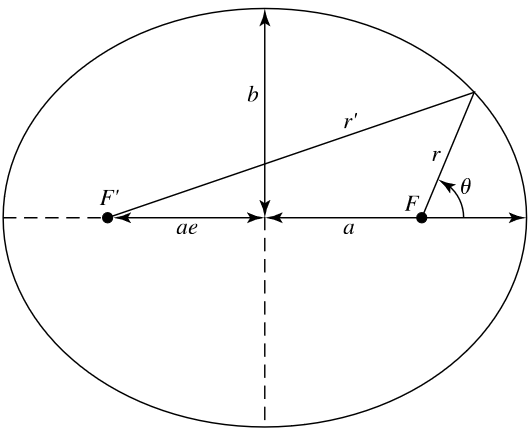
\includegraphics[width=0.45\textwidth]{ellipseGeometry.png}
\end{center}
Geometrically, the ellipse is characterized by its \textbf{semimajor axis} $a$, \textbf{semiminor axis} $b$, and \textbf{eccentricity} $e$.
There's a pretty simple relationship between these three quantities!
Let $r$ be the distance from the planet to the star; by the Pythagorean theorem, at a point on the semiminor axis,
\[ r^2 = b^2 + a^2e^2. \]
Recall that an ellipse is defined by the equation $r + r' = 2a$, where $r'$ is the distance from a point to the other (empty) focus.
In this case, $r = r'$, so $r = a$ and
\[ \boxed{b^2 = a^2 (1 - e^2)}. \]
There's another relationship that we can derive, one that gives the planet's distance from the sun given any $\theta$ on the ellipse (as defined in the figure).
Again applying the Pythagorean theorem, this time at the point draw above:
\begin{align*}
    r'^2 &= (r \sin \theta)^2 + (2ae + r \cos \theta)^2 \\
    r'^2 &= r^2 + 4ae(ae + r \cos \theta)
\end{align*}
Substituting the definition of an ellipse $r' = 2a - r$ and solving for $r$ gives
\[ \boxed{r = \frac{a(1 - e^2)}{1 + e \cos \theta}, \quad 0 \leq e < 1}. \]
This equation actually applies to all of the different conic sections, just with different values of $e$!
In the special case $e = 0$ we get a circle, which reveals that the circle is just a special type of ellipse in which the foci coincide.
(In fact, the area of an ellipse can be expressed as $A = \pi ab$, which easily reduces to that of a circle by taking $a = b = r$.)
Setting $e=1$ and $e > 1$ gives parabolas and hyperbolas, respectively.
Each of these four curves describes a different type of celestial motion (we'll return to this soon).

Now, the orbital elements $a$, $e$, and $\theta$ (also called $f$) are enough to characterize an ellipse and an object's position on it.
However, it says nothing about the ellipse's orientation in space.
So we introduce three more orbital elements to describe it:
\begin{itemize}
    \item The inclination $i$ is the angle between the orbital plane and a reference plane, like the equatorial plane.
    \item The longitude of ascending node $\Omega$ is the horizontal angle (longitude) from a point in the reference plane, like the vernal equinox, to the point at which the orbit intersects the reference point going northward (the ascending node).
    \item The argument of pericenter $\omega$ is the angle (argument) from the ascendng node to pericenter.
\end{itemize}
Unsurprisingly, there is a one-to-one mapping between the initial conditions $\mbf{r}_0, \mbf{v}_0$ and the six obital elements we've defined; we won't describe that mapping here.
What we \textit{will} describe, however, is the connection between some of these orbital elements to the system's main conserved quantities.

Since gravity exerts no torque on the planet, the angular momentum $\mbf{L} = m \mbf{r} \times \mbf{v}$ is conserved.
It will be useful for us to define the \textbf{specific angular momentum}---that is, angular momentum per unit mass---as
\[ \mbf{h} = \mbf{r} \times \mbf{v}. \]
It turns out that, by solving the initial-value problem that governs the plane's dynamics, we can write
\[ r = \frac{h^2/GM_\star}{1 + e \cos \theta}. \]
(This is another one of those things that we'll take for granted.)
So we have the relationship
\[ \frac{h^2}{GM_\star} = a (1 - e^2) \implies \boxed{h^2 = GM_\star a (1 - e^2)}. \]
Similarly, the energy $\mathcal{E} = \frac{1}{2}v^2 - \frac{GM_\star}{r}$ is conserved since gravity is the only force acting on the planet, and we can define the \textbf{specific energy}
\[ \mathcal{E} = \frac{1}{2}v^2 - \frac{GM_\star}{r}. \]
We can derive a relationship for this one on our own.
Consider the state of the planet at pericenter---it has position $a(1 - e)$ and velocity $v_p$.
We can find an expression for $v_p^2$ using the specific angular momentum, noting that the position and velocity vectors are orthogonal at pericenter:
\[ h = a (1 - e) \cdot v_p \implies v_p = \frac{h}{a (1 - e)}. \]
Using this to calculate the specific energy:
\begin{align*}
    \mathcal{E} &= \frac{1}{2} \frac{h^2}{a^2 (1-e)^2} - \frac{GM_\star}{r} \\
    &= \frac{GM_\star a (1 - e^2)}{2a^2 (1-e)^2} - \frac{GM_\star}{a (1-e)} \\
    \Aboxed{\mathcal{E} &= -\frac{GM_\star}{2a}}.
\end{align*}

We're now in a position to derive Kepler's other laws with ease.

\textbf{Kepler's second law} states that the rate at which a planet's orbit sweeps out area is constant.
To show this, consider the triangle that the planet sweeps out in an infinitesimal time $dt$.
\begin{center}
    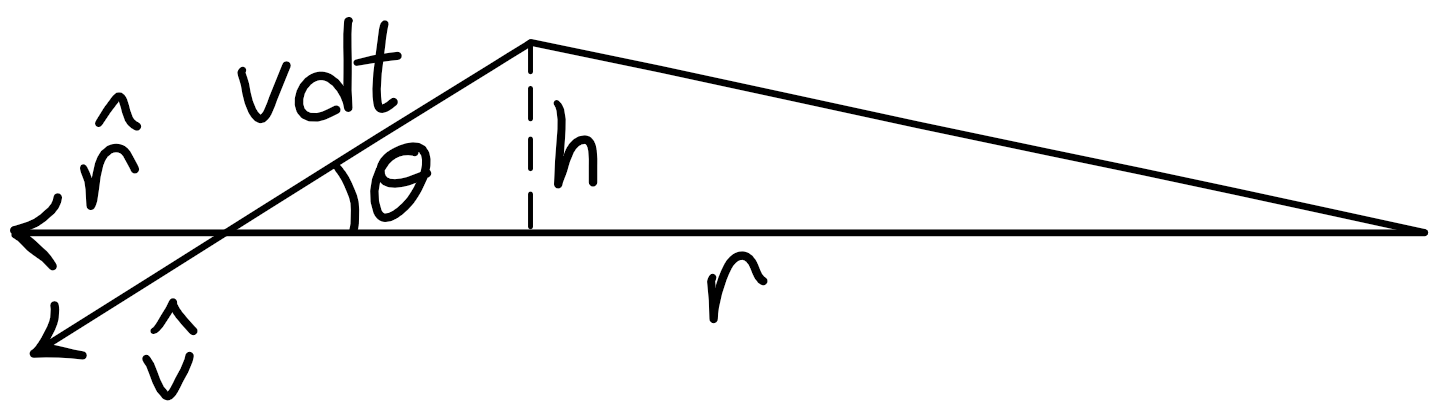
\includegraphics[width=0.35\textwidth]{sweptTriangle.png}
\end{center}
If the area of this triangle is $dA$, then
\[ dA = \frac{1}{2} r (v \,dt \,\sin \theta) \implies \frac{dA}{dt} = \frac{rv \sin \theta}{2}. \]
So $\boxed{dA/dt = h/2}$, which is constant!

\textbf{Kepler's third law} gives a relationship between a planet's orbital period and its semimajor axis.
For this one, we simply use the fact that
\[ P = \frac{A_\textrm{ellipse}}{dA/dt} = \frac{\pi ab}{h/2} = \frac{2 \pi a (a \sqrt{1 - e^2})}{\sqrt{GM_\star a (1-e^2)}} = \frac{2 \pi}{\sqrt{GM}} a^{\frac{3}{2}}. \]
Squaring gives
\[ \boxed{P^2 = \frac{4 \pi^2}{GM_\star} a^3}. \]
That's it for Kepler's laws!
These are valid for bound orbits, which are ones that keep the planet (or other astronomical object) within the grasp of a parent star.

To determine if an orbit is bound or unbound we look at the amount of energy an object possesses.
If its energy is positive (or zero) then it will always have \textit{some} kinetic energy, so its orbit is unbound.
Negative energies, on the other hand, correspond to bound orbits.
More specfically:

\begin{center}
\begin{tabular}{c|c|c|c|c}
    Shape & Bound? & Energy & Semimajor Axis & Eccentricity \\ \hline
    Hyperbola & No & $E > 0$ & $a < 0$ & $e > 1$ \\
    Parabola & No & $E = 0$ & $a = \infty$ & $e = 1$ \\
    Ellipse & Yes & $E < 0$ & $a > 0$ & $0 \leq e < 1$ \\
    Circle & Yes & $E < 0$ & $a > 0$ & $e = 0$
\end{tabular}
\end{center}

Another important property of energy in these systems is given by the \textbf{virial theorem}.
Recall how, for circrular orbits,
\[ \frac{GM_\star}{r^2} = \frac{v^2}{r}, \]
so $v^2 = GM/r$.
This gives the kinetic energy
\[ K = \frac{GM_\star m}{2r} = -\frac{U}{2}. \]
In a slightly more general sense, we can make the following statement for any gravitationally bound system in equilibrium:
\[ \boxed{\left< K \right> = -\frac{\left< U \right>}{2}}, \]
where quantities in the angle brackets are time averages (usually over one period).

\subsection*{The General Two-Body Problem}
Now we can tackle the general two-body problem---that is, the two-body problem with two finite masses $m_1$ and $m_2$
Because the system's total momentum is conserved, our analysis will be easiest in the center-of-mass reference frame.

Place the center of mass at the origin of our coordinate system.
The position vectors of the masses are $\mbf{r}_1$ and $\mbf{r}_2$, respectively.
But the dynamics of the two-mass system really only depend on the displacement $\mbf{r} = \mbf{r}_2 - \mbf{r}_1$, so it will be useful to relate each position vector to the displacement.
This is done pretty easily by substituting the proper information into the equation $(m_1\mbf{r}_1 + m_2\mbf{r}_2)/M = 0$, where $M = m_1 + m_2$.
\[ \mbf{r}_1 = \frac{m_2}{M} (-\mbf{r}), \quad \mbf{r}_2 = \frac{m_1}{M} \mbf{r}. \]
We can actually use this to greatly simplify our problem!
First, we write two equivalent expressions for the quantity $m_2\ddot{\mbf{r}}_2 - m_1\ddot{\mbf{r}}_1$.
\begin{align*}
    m_2\ddot{\mbf{r}}_2 - m_1\ddot{\mbf{r}}_1 &= m_2 \left( \frac{m_1}{M}\ddot{\mbf{r}} \right) - m_1 \left( \frac{m_2}{M} (-\ddot{\mbf{r}}) \right) & m_2\ddot{\mbf{r}}_2 - m_1\ddot{\mbf{r}}_1 &= -m_2 \frac{Gm_1}{r^2}\hat{r} - m_1 \frac{Gm_2}{r^2}\hat{r} \\
    &= \frac{2m_1m_2}{M}\ddot{\mbf{r}} & &= -\frac{2Gm_1m_2}{r^2}\hat{r}
\end{align*}
Therefore,
\[ \frac{m_1m_2}{M}\ddot{\mbf{r}} = -\frac{Gm_1m_2}{r^2}\hat{r}. \]
To write this a little more suggestively, we can define the \textbf{reduced mass} $\mu = \frac{m_1m_2}{m_1 + m_2}$ to get
\[ \boxed{\mu \ddot{\mbf{r}} = -\frac{GM\mu}{r^2}\hat{r}}. \]
Notice how this is the equation of motion for a body with mass $\mu$ orbiting around a fixed mass $M$ at a distance $r$.
We've just taken our general two-body problem and reduced it to an equivalent one-body problem!
So all of the equations that we've derived for the restricted two-body problem also apply here, after a few substitutions.

We don't need to change anything about the eccentricity of the orbit.
It should make sense for example, that a highly eccentric two-body system would stay highly eccentric in our equivalent reduced model.
To see what happens to the semimajor axis, we exploit the fact that the distance $r$ between $\mu$ and $M$ is the sum of the objects' distances to the center of mass.
At perihelion we have
\begin{align*}
    r &= r_1 + r_2 \\
    a(1-e) &= a_1(1-e) a_2(1-e) \\
    a &= a_1 + a_2,
\end{align*}
Finally, we replace all instances of $M_\star$ with $M$.
This gives us the set of substitutions
\begin{empheq}[box=\fbox]{align*}
    r &\to r_1 + r_2 \\
    a &\to a_1 + a_2 \\
    M_\star &\to M
\end{empheq}
As a corollary, we can also derive a more direct pair of relationships for the semimajor axes (using the fact that $r_1 = a_1$ and $r_2 = a_2$ on the semiminor axis):
\[ a_1 = \frac{m_2}{M}a, \quad a_2 = \frac{m_1}{M}a. \]
We also have simple equations for the kinetic energy and angular momentum, both in the center-of-mass frame.
\begin{empheq}[box=\fbox]{align*}
    E &= \frac{1}{2} \mu v^2 - \frac{GM-\mu}{r^2} \\
    \mbf{L} &= \mu (\mbf{r} \times \mbf{v}),
\end{empheq}
where $\mbf{v} \equiv d\mbf{r}/dt$.
Lastly, we give an alternative relation between $\mbf{r}$ and the position vectors.
\[ \boxed{\mbf{r}_1 = \frac{\mu}{m_1} (-\mbf{r}), \quad \mbf{r}_2 = \frac{\mu}{m_2} \mbf{r}}. \]

\subsection*{Detection of Exoplanets}
As an application, let's discuss the detection of planets in extrasolar systems.
The most obvious way of doing this is via direct imaging.
We cover up the light coming from a star so that its brightness doesn't overpower that of any orbiting bodies, and we see what we can see.
(This method isn't perfect since some light diffracts around the blockage, but good software will be able to filter this out.)
This generally only works with very large planets with very large orbits.

Alternatively, we can use our newfound knowledge of orbital mechanics!
Suppose we have a planet-star system orbiting around a common center of mass; let $\mbf{v}_\star$ be the star's orbital velocity and let $\mbf{v}_r$ be the component of this velocity that is in the observer's direction.
\begin{center}
    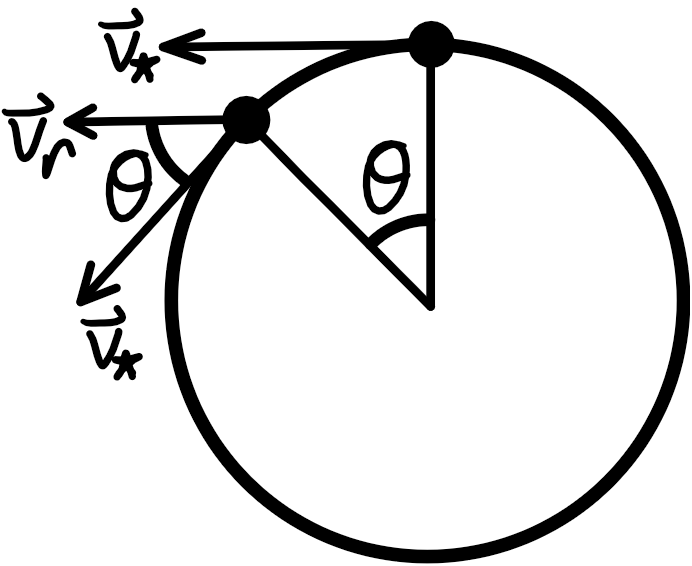
\includegraphics[width=0.3\textwidth]{exoplanetDoppler.png}
\end{center}
As the star moves toward or away from us, the light it emits experiences a Doppler shift---it is blueshifted and redshifted, respectively.
For $v_r \ll c$, this shift is quantified by
\[ \frac{\lambda_\textrm{obs} - \lambda_\textrm{em}}{\lambda_\textrm{em}} = \frac{\Delta \lambda}{\lambda_\textrm{em}} = \frac{v_r}{c}. \]
So clearly $v_r$ is an important quantity.
We can relate it to known values using some simple trigonometry!
If $\theta$ is the angle between $\mbf{v}_\star$ and $\mbf{v}_r$, then we have $v_r = v_\star \cos \theta$.
If we define a time $t=0$ at the angle $\theta=0$, then the relationship is
\[ v_r = v_\star \cos \left( \frac{2\pi t}{P} \right), \]
where $P$ is the orbital period of the star.
But in general, we won't be looking at planetary systems edge-on, but rather at some inclination $i$.
If $i=90^\circ$ corresponds to the edge-on view, then we have
\[ \boxed{v_r = (v_\star \sin i) \cos \left( \frac{2\pi t}{P} \right)}. \]
From here we can do a couple of things.
For one, we could observe the change in the star's spectrum over time to determine its mass; we'll do more of that later on.
But assuming we have the result of this analysis, we could also determine the planet's mass $m_p$ with the knowledge we have now!

Let's take a look at our observables.
We have the maximum radial velocity $v_\textrm{max} = v_\star \sin i$, the orbital period $P$, and the mass $M_\star$ of the star.
We also have the simple $d = rt$ relationship
\[ v_\star = \frac{2 \pi a_\star}{P}. \]
Since $a_\star = (m_p / M_\textrm{tot}) a$, where $a$ is the reduced-mass semimajor axis, this is equivalent to
\[ v_\star = \frac{2\pi}{P} \frac{m_p}{M_\textrm{tot}} a = \frac{2\pi}{P} \frac{m_p}{M_\textrm{tot}} \left( \frac{P^2 GM_\textrm{tot}}{4 \pi^2} \right)^{1/3}, \]
where the last step follows from Kepler's third law.
When we set this equal to $v_\textrm{max} / \sin i$ and take $m_p \ll M_\star$, we get
\[ \boxed{m_p \sin i = v_\textrm{max} \left( \frac{PM_\star^2}{2\pi G} \right)}. \]
Everything on the right side of this equation is an observable quantity!
Since $\sin i$ never exceeds 1, this expression gives us a lower bound for the mass of the exoplanet.

\section{Measures of Brightness}
We've spent plenty of time analyzing the positions and motions of objects in the sky.
Now we'll turn to the question of how bright something is, in both relative terms and absolute ones.

\subsection*{Luminosity, Flux, and Magnitude}
The most fundamental measure of brightness we can define is the \textbf{luminosity} $L = dE / dt$, which is simply the energy emitted per unit time.
We could call this ``power'' like we do elsewhere in physics, but we normally don't to distinguish the production of radiative energy from other phenomena.

When objects like stars give off energy, they do so in a spherically symmetric manner.
So it will be useful to define the \textbf{flux}
\[ \boxed{F_\textrm{obs} = \frac{dE}{dt \,dA} = \frac{L}{4 \pi d^2}}, \]
which changes as a function of the distance $d$ from the source.
This flux is not the same as the quantity we defined in E\&M!
We can interpret $F$ as a measure of ``power'' per unit area on some radius-$d$ sphere.
If we take the radius of this sphere to simply be that of the star we're looking at, $R$, then we get another absolute quantity: the \textbf{emitted flux}
\[ F_\textrm{em} = \frac{L}{4 \pi R^2}. \]
The relationship between the observed and emitted flux is simply $F_\textrm{obs} = F_\textrm{em} (R / d)^2$.

These two quantites we've defined are relatively modern ones in the broader context of astronomy.
In ancient times observers had only their logarithmic eyes to go off of, and all of their observations were relative rather than absolute.
The \textbf{magnitude scale}, devised in ancient Greece, is defined in modern terms as follows.
If we have two objects with fluxes $F_1$ and $F_2$, then their magnitudes $m_1$ and $m_2$ are
\[ \boxed{m_1 - m_2 = 2.5 \log_{10} \frac{F_2}{F_1}}. \]
A few important things to note about this scale.
Also:
\begin{itemize}[topsep=0pt]
    \item This definition is innherently relative---in isolation it is only meaningful when we compare the magnitudes of two stars.
    So if we want to assign each object its own unique magnitude we must agree on a standard value of $F$ that corresponds to $m=0$; Vega is the usual choice for this.

    \item This definition is also relative in another sense: it depends on the distance from the object, just like $F$.
    To distinguish it from the absolute magnitude (which we'll define shortly), we call $m$ an apparent magnitude.

    \item Finally, the magnitude scale runs opposite of how we might expect it to.
    Brighter stars have lower magnitudes than dimmer ones.
    This feels weird, but its origins are logical---it's a consequence of using zero as a base line for the brightest stars in the sky and going from there.
\end{itemize}
Now, if apparent magnitude is defined in terms of flux, we might expect that the absolute magnitude of an object is related to its luminosity.
Specifically, if we define the \textbf{absolute magnitude} $M$ as the apparent magnitude of an object seen at a distance of $d = 10 \text{ pc}$, we get
\begin{align*}
    M_1 - M_2 &= 2.5 \log_{10} \left( \frac{F_2 (d)}{F_1 (d)} \right) \\
    &= 2.5 \log_{10} \left( \frac{L_2}{4 \pi d^2} \cdot \frac{L_1}{4 \pi d^2} \right) \\
    \Aboxed{M_1 - M_2 &= 2.5 \log_{10} \frac{L_2}{L_1}}
\end{align*}
Again, we usually use Vega as our standard $M=0$.
We can take advantage of our two definitions here to approximate the distance to an object!
We know how to measure $m$ directly, and we can often make a pretty good guess for $M$ based on other characteristics (we'll see how later).
The distance $d$ to the object is related to these quantities by the equation
\begin{align*}
    m - M &= 2.5 \log_{10} \left( \frac{F (10 \text{ pc})}{F (d)} \right) \\
    &= 2.5 \log_{10} \left( \frac{L}{4 \pi (10 \text{ pc})^2} \cdot \frac{4\pi d^2}{L} \right) \\
    \Aboxed{m - M &= 5 \log_{10} \frac{d}{10 \text{ pc}}}
\end{align*}
This is often called the \textbf{distance modulus}.

\subsection*{Solid Angles and Intensity}
All of our definitions here are great for point sources that emit light isotropicallly in all directions.
But what if this isn't the case?
As a step toward accounting for this, we'll define a quantity that, in a sense, indicates direction: the \textbf{solid angle} $\Omega$.

A solid angle is just an angle in three dimensions.
Just like how we have $d\theta = ds/r$ in two dimensions, in 3D we have
\[ \boxed{d \Omega = \frac{dA}{r^2} = d\theta \sin \theta \,d\varphi}, \]
where $dA = r\,d\theta \cdot r \sin \theta \,d\phi$ is a differential area on the celestial sphere.
($\varphi$ is the angle in the $xy$-plane while $\theta$ is the angle from the $z$-axis.)
Solid angles are measured in steradians (sr) which, like radians, \textit{technically} aren't real units but we usually write them down for bookkeping purposes.
We could show, by integrating $d\Omega$ over the entire celestial sphere, that there are $4\pi \text{ sr}$ in a full sphere.

Now we're ready to define the ``directional brightness'' that we initially desired.
Taking into account that an observer may detect incoming light at an angle $\theta$ (where $\theta = 0$ corresponds to observing the light straight-on), we define the \textbf{intensity} as
\[ \boxed{I = \frac{dE}{dt \, d\Omega \, dA \cos \theta}}, \]
where $dA \cos \theta$ is the differential normal area of some detector.
This is the energy detected (or emitted!) per unit time, per unit solid angle, per unit normal area.

There's a pretty straightforward relationship between $F$ and $I$ that we can determine just by inspecting their definitions:
\[ F = \int_{\Omega}^{} I \cos \theta \,\Omega. \]
The extra factor of $\cos \theta$ ensures that light incident at a relatively large $\theta$ contributes less to the overall flux than light from other directions.
There are a couple of assumptions that we can often take to make the integral much easier.
First, if the observer is looking directly at the object then $\theta \approx 0$ for all light, so $\cos \theta \approx 1$ and
\[ F \approx \int_{\Omega}^{} I \,d\Omega = I \Omega. \]
If the sky is uniformly bright, then $I$ is constant and the flux from all light is
\[ F = \int_{0}^{\pi / 2} I \cos\theta (\sin\theta \,d\theta) \int_{0}^{2\pi}d\varphi = \pi I. \]
This result is useful in determining the total (observed) emitted flux from an isotropic emitter, like we'd see on the surface of a star!

\subsection*{Speciific Brightness}
We can split up each of our quantities in one more way.
We're often only concerned with the brightness of an object in one wavelength or frequency.
For example, we can define the specific luminosity
\[ L_\lambda = \frac{dL}{d\lambda} \,\text{ or } L_\nu = \frac{dL}{d\nu}, \]
which are not equivalent but communicate the same sort of thing.
They're characterized by the integrals
\[ L = \int_{0}^{\infty} L_\lambda \,d\lambda = \int_{0}^{\infty} L_\nu \,d_\nu, \]
respectively, which suggests the relationship
\[ L_\lambda |d\lambda| = L_\nu |d\nu| \]
and thus
\[ \boxed{L_\nu = \left| \frac{d\lambda}{d\nu} \right| L_\lambda} \implies \boxed{\nu L_\nu = \lambda L_\lambda}. \]
We can do something similar with specific flux and luminosity, which is often useful.

\section{Blackbody Radiation}
\subsection*{Blackbody Radiation}
Armed with these definitions, we can get back into some astrophysics!
We'll start by talking about blackbodies, which are objects that are completely opaque, nonreflective, and in thermal equilibrium.
Of course, such a body does not exist, but this model approximates the properties of objects like stars to a surprising degree.

For a blackbody at a temperature $T$, one might derive its specific intensity at different wavelengths (or frequencies).
That's a problem for statistical mechanics, though, so we'll just quote the result, which is called the \textbf{Planck function}.
\[ \boxed{I_\lambda = B_\lambda = \frac{2hc^2 / \lambda^{5}}{e^{hc / kT\lambda} - 1} \qquad\qquad I_\nu= B_\nu = \frac{2h\nu^3 / c^2}{e^{h\nu / kT} - 1}} \]
Here $k = k_B$ is the Boltzmann constant, $h$ is the Planck constant, and $c$ is the speed of light in a vacuum.
Like with luminosity, we can convert between these quantities using the equation $I_\lambda |d\lambda| = I_\nu |d\nu|$.

Notice that an object's Planck function depends \textit{only} on its temperature.
Objects at higher temperatures have higher intensities at all wavelengths, but their peak wavelengths are lower than cooler counterparts.
The plot below illustrates this at three different temperatures (incuding the Sun's, at 5777 K).
\begin{center}
    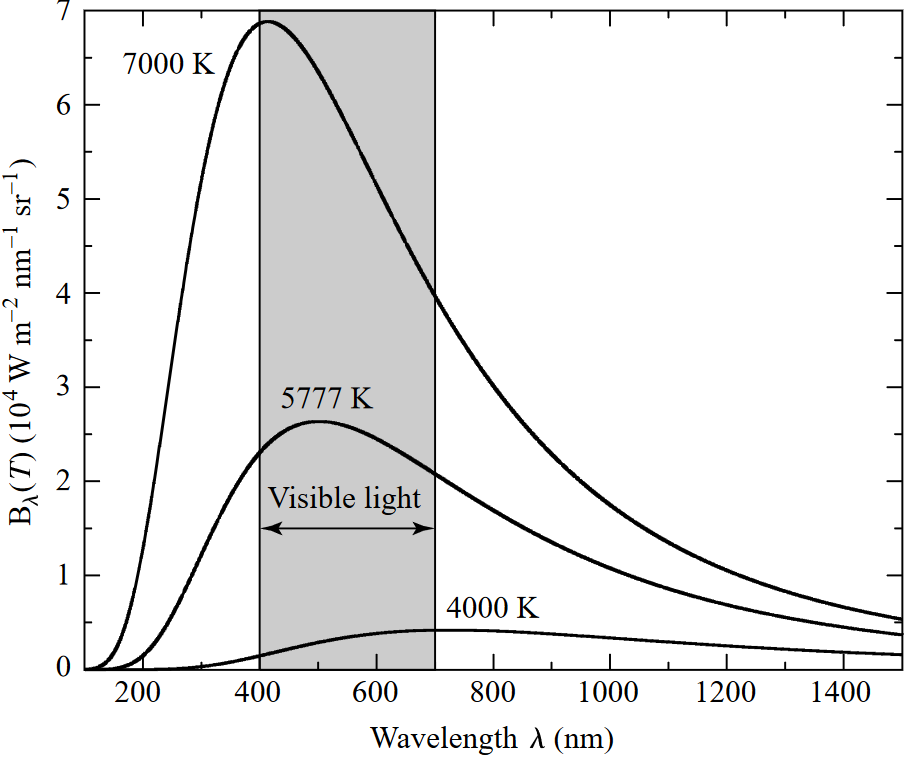
\includegraphics[width=0.55\textwidth]{blackbodyCurves.png}
\end{center}
To determine what this peak wavelength is, one could solve the equation $dB_\lambda / d\lambda = 0$ to find that
\[ \boxed{\lambda_\textrm{peak} = \frac{b}{T}}, \]
where $b = 0.29 \text{ cm K}$.
This is called \textbf{Wien's displacement law}, and it explains why bodies with different temperatures appear to be different colors!

When we integrate across all wavelengths, we get the total intensity
\begin{align*}
    I = B &= \int_{0}^{\infty} B_\lambda d\lambda \\
    &= \int_{0}^{\infty} \frac{2hc^2 d\lambda}{\lambda^{5} (e^{hc/kT\lambda} - 1)} \\
    I = B &= \frac{\sigma T^{4}}{\pi},
\end{align*}
where $\sigma = (2\pi^{5} k^{4}) / (15h^{3} c^2)$ is the Stefan-Boltzmann constant.
Since $F = \pi I$ for an isotropic sky, the emitted flux from a blackbody is
\[ \boxed{F_\textrm{em} = \sigma T^{4}}. \]
This gives the total luminosity
\[ \boxed{L = 4\pi R^2 \sigma T^{4}}, \]
where $R$ is the radius of the blackbody.
This equation is particularly useful when dealing with thermal equilibria, which are characterized by $L_\textrm{abs} = L_\textrm{em}$.

\subsection*{Albedo and Color Magnitudes}
Now, what happens when we relax one of our assumptions by allowing our bodies to be reflective?
We'll define \textbf{albedo} $a$ as the fraction of incident light that is reflected rather than absorbed.
This fraction is generally a function of wavelength.
Assuming the body is still in thermal equilibrium, emitted light must exactly match absorbed light at all wavelengths.
Expressed in terms of wavelength,
\begin{align*}
    I_\textrm{abs}(\lambda) &= \left[ 1 - a(\lambda) \right] I_\textrm{inc} \\
    I_\textrm{em}(\lambda) &= \left[ 1 - a(\lambda) \right] B_\lambda
\end{align*}
We might use this information to estimate the equilibrium temperature of a planet by setting $I_\textrm{abs} = I_\textrm{em}$ and considering only the wavelengths of maximum absorption and emission.
This approximation, however, does not account for atmospheres and so may be cooler than reality.

We now have several different ways of estimating temperature from a blackbody spectrum, but they all require information spanning a wave range of wavelengths, which can be quite challenging to obtain.
We'll give one much cruder, but still effective, method for measuring these temperatures.

Thus far we've been talking about bolometric (total) magnitudes, that is, magnitudes across all wavelengths.
However, telescopes make observations through filters for very small bands of wavelengths (like Ultraviolet, Blue, Visual, Red, and Infrared).
The flux through a filter $X$ is given by
\[ F_X = \int_{0}^{\infty} F_\lambda S_X(\lambda) \,d\lambda, \]
where $S_X(\lambda)$ is the probability that a photon of wavelength $\lambda$ passes through filter $X$.
We use this to define the \textbf{color magnitude} for $X$:
\[ m_{X,1} - m_{X,2} = 2.5 \log_{10} \left( \frac{F_{X,2}}{F_{X,1}} \right). \]
But as long as the specific flux $F_\lambda$ doesn't change too abruptly in $X$, we can write this as
\[ \boxed{X_1 - X_2 = 2.5 \log_{10} \left( \frac{F_{\lambda, 2} (\lambda_X)}{F_{\lambda, 1} (\lambda_X)} \right)}, \]
where $\lambda_X$ is the maximum wavelength in $X$ and the magnitudes are denoted by $X_1$ and $X_2$.

We can take advantage of this definition to characterize the temperatures of stars!
Start with the color magnitudes in the $V$ and $B$ bands:
\begin{align*}
    V - V_0 &= 2.5 \log_{10} \left( \frac{F_{\lambda_0} (\lambda_V)}{F_\lambda (\lambda_V)} \right) \\
    B - B_0 &= 2.5 \log_{10} \left( \frac{F_{\lambda_0} (\lambda_B)}{F_\lambda (\lambda_B)} \right)
\end{align*}
Subtracting these equations,
\begin{align*}
    B - V &= 2.5 \log_{10} \left( \frac{F_{\lambda_0} (\lambda_B)}{F_{\lambda_0} (\lambda_V)} \cdot \frac{F_{\lambda} (\lambda_V)}{F_{\lambda} (\lambda_B)} \right) \\
    &= 2.5 \log_{10} \left( \frac{F_{\lambda} (\lambda_V)}{F_{\lambda} (\lambda_B)} \right) + 2.5 \log_{10} \left( \frac{F_{\lambda_0} (\lambda_B)}{F_{\lambda_0} (\lambda_V)} \right)
\end{align*}
But the second is the B-V of Vega, which we define to be zero.
This gives us the \textbf{color index}
\[ \boxed{B - V = 2.5 \log_{10} \left( \frac{F_{\lambda} (\lambda_V)}{F_{\lambda} (\lambda_B)} \right) = 2.5 \log_{10} \left( \frac{L_V}{L_B} \right)}. \]
Notice that the color magnitude is a function only of temperature, not distance!
Also note that a larger $F_\lambda (\lambda_B)$ compared to $F_\lambda (\lambda_V)$ corresponds to a higher temperature, so B-V decreases with increasing temperature.

The Hertzsprung-Russel (H-R) diagram is a plot of luminosity against color index.
There's a very prominent negative correlation of stars called the main sequence.
As it turns out, the location of a given star on the main sequence is entirely determined by its mass---the higher the mass, the higher the position on the main sequence (brighter but cooler).
There are some pretty tight empirical correlations between the main stellar parameters on the main sequence.
Specifically:
\[ \frac{L}{L_\odot} \approx \left( \frac{M}{M_\odot} \right)^{3.5} \qquad \frac{R}{R_\odot} \approx \left( \frac{M}{M_\odot} \right)^{0.7} \qquad \frac{T}{T_\odot} \approx \left( \frac{M}{M_\odot} \right)^{0.56} \]
We'll spend some time building stellar models in an attempt to understand the origins of empirical relations like these.

% TODO: measure what to infer what?

\end{document}